\documentclass[t,12pt]{beamer}
%
% Packages pour le français
\usepackage[T1]{fontenc}
\usepackage[utf8]{inputenc}
\usepackage[frenchb]{babel}
%
% pour un pdf lisible à l'écran
% il y a d'autres choix possibles
\usepackage{pslatex}
\usepackage{listings}
\usepackage{graphicx}
%
% pour le style et couleurs
\usetheme{Boadilla}
%
% contenu de la page de titre
\title{Présentation des langages fonctionnel}
\subtitle{Historique et définition}
\author{Jacques-Pascal Deplaix}
\date{\oldstylenums{Février 2013}}
%
% Fin du préambule
%
\begin{document}

\defverbatim[colored]\ocamlFact{
  \begin{lstlisting}[language=Caml]
    let rec fact = function
      | 0 -> 1
      | x -> x * fact (x - 1)
  \end{lstlisting}
}
\defverbatim[colored]\haskellFact{
  \begin{lstlisting}[language=Caml]
    fact 0 = 1
    fact x = x * fact (x - 1)
  \end{lstlisting}
}
\defverbatim[colored]\lispFact{
  \begin{lstlisting}[language=Python]
    (defun fact (n)
      (if (< n 2)
	  1
	(* n (fact (- n 1)))))
  \end{lstlisting}
}
\defverbatim[colored]\erlangFact{
  \begin{lstlisting}[language=Caml]
    fact(0) -> 1;
    fact(N) when N > 0 -> N * fact(N - 1).
  \end{lstlisting}
}
\defverbatim[colored]\pythonExample{
  \begin{lstlisting}[language=Python]
    x = list(map(lambda x: x * 2,
		 [x + 1 for x in range(10)]))
  \end{lstlisting}
}
\defverbatim[colored]\rubyExample{
  \begin{lstlisting}[language=Ruby]
    x = [1, 2, 3].map {|x| x * 2}
  \end{lstlisting}
}
\defverbatim[colored]\jsExample{
  \begin{lstlisting}[language=Caml]
    [1, 2, 3].map(function(x) {return x * 2;})
  \end{lstlisting}
}
\defverbatim[colored]\valaExample{
  \begin{lstlisting}[language=Java]
std::qsort(list.begin(), list.end(),
	   [](const MyStruct&a,const MyStruct&b) {
	     auto m_a = a.member;
	     return m_a < b.member;
	   });
  \end{lstlisting}
}

\frame{\titlepage}

\begin{frame}
  \tableofcontents
\end{frame}

\section{Quelques définitions}
\begin{frame}
  \frametitle{Quelques définitions}
  \framesubtitle{Qu'est ce que le paradigme fonctionnel ?}

  \begin{block}{Les bases}
    \begin{itemize}
      \item Lambda calcul
    \end{itemize}
  \end{block}

  \begin{block}{Propriétés}
    \begin{itemize}
      \item Non-mutablilité
      \item Fonctions de premier ordre/ordre supérieur
      \item Récursion
      \item Lambda/Fonctions anomyme
      \item Currification et application partielle
    \end{itemize}
  \end{block}

\end{frame}

\section{Les langages}
\subsection{Lisp}
\begin{frame}
  \frametitle{Lisp}
  \framesubtitle{Lots of Irritating Superfluous Parentheses}

  \begin{exampleblock}{Un exemple de factorielle}
    \lispFact
  \end{exampleblock}

  \begin{block}{Avancées majeurs}
    \begin{itemize}
      \item La récusion
      \item Un garbage collector (GC)
      \item Les fonctions de premier ordre/ordre supérieur
      \item Les lambda/Fonctions anomyme
    \end{itemize}
  \end{block}
\end{frame}

\subsection{ML/Caml/OCaml}
\begin{frame}
  \frametitle{ML/Caml/OCaml}
  \framesubtitle{Des vrais types}

  \begin{exampleblock}{Un exemple de factorielle}
    \ocamlFact
  \end{exampleblock}

  \begin{block}{Avancées majeurs}
    \begin{itemize}
      \item Des types
      \item L'inférence de types
      \item Polymorphisme paramètrique
    \end{itemize}
  \end{block}
\end{frame}

\subsection{Haskell}
\begin{frame}
  \frametitle{Haskell}
  \framesubtitle{Pour quelques monades de plus}

  \begin{exampleblock}{Un exemple de factorielle}
    \haskellFact
  \end{exampleblock}

  \begin{block}{Avancées majeurs}
    \begin{itemize}
      \item Les classes de types
      \item L'évaluation paresseuse
      \item Les listes en comprehension
      \item Les monades
    \end{itemize}
  \end{block}
\end{frame}

\subsection{Erlang}
\begin{frame}
  \frametitle{Erlang}
  \framesubtitle{Concurrence everywhere}

  \begin{exampleblock}{Un exemple de factorielle}
    \erlangFact
  \end{exampleblock}

  \begin{block}{Avancées majeurs}
    \begin{itemize}
      \item Le modèle d'acteur (multi-processus par passage de messages)
    \end{itemize}
  \end{block}
\end{frame}

\section{Un petit historique}
\begin{frame}
  \frametitle{Un petit historique}
  \framesubtitle{Un peu d'histoire…}
  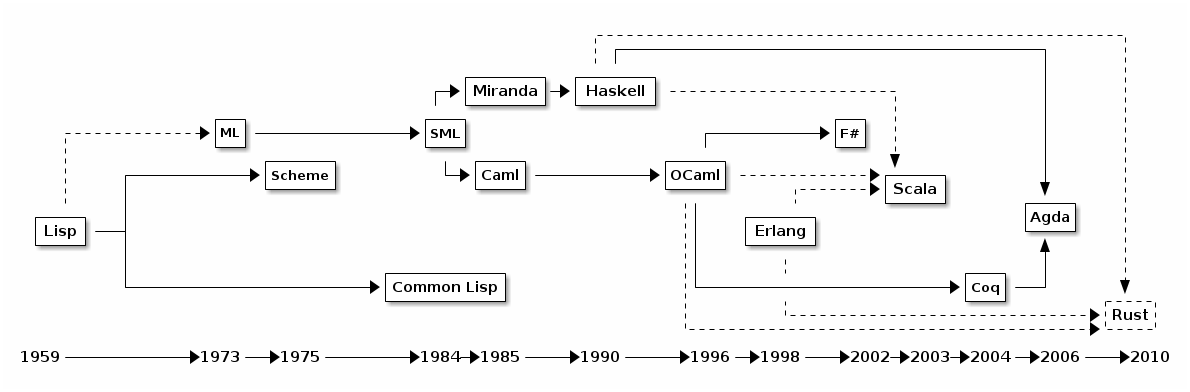
\includegraphics[scale=0.29]{history.png}
\end{frame}

\section{Impact dans les autres langages}
\begin{frame}
  \frametitle{Impact dans les autres langages}
  \framesubtitle{Evil- -}

  \begin{block}{Fonctionnalités hérité}
    \begin{itemize}
      \item Fonctions anomyme
      \item Les fonctions d'ordre supérieur
      \item Les listes en comprehension
      \item Typage et inférence
    \end{itemize}
  \end{block}
\end{frame}

\subsection{Python}
\begin{frame}
  \frametitle{Python}
  \framesubtitle{Un exemple}

  \begin{exampleblock}{Un exemple de programme fonctionnel en Python}
    \pythonExample
  \end{exampleblock}

  \begin{block}{Fonctionnalités hérité}
    \begin{itemize}
      \item Fonctions anomyme
      \item Les fonctions d'ordre supérieur
      \item Les listes en comprehension
    \end{itemize}
  \end{block}
\end{frame}

\subsection{Ruby}
\begin{frame}
  \frametitle{Ruby}
  \framesubtitle{Un exemple}

  \begin{exampleblock}{Un exemple de programme fonctionnel en Ruby}
    \rubyExample
  \end{exampleblock}

  \begin{block}{Fonctionnalités hérité}
    \begin{itemize}
      \item Fonctions anomyme
      \item Les fonctions d'ordre supérieur
    \end{itemize}
  \end{block}
\end{frame}

\subsection{Javascript}
\begin{frame}
  \frametitle{Javascript}
  \framesubtitle{Un exemple}

  \begin{exampleblock}{Un exemple de programme fonctionnel en Javascript}
    \jsExample
  \end{exampleblock}

  \begin{block}{Fonctionnalités hérité}
    \begin{itemize}
      \item Fonctions anomyme
      \item Les fonctions d'ordre supérieur
    \end{itemize}
  \end{block}
\end{frame}

\subsection{C++/Csharp/Vala}
\begin{frame}
  \frametitle{C++/Csharp/Vala}
  \framesubtitle{Un exemple}

  \begin{exampleblock}{Un exemple de programme fonctionnel en C++}
    \valaExample
  \end{exampleblock}

  \begin{block}{Fonctionnalités hérité}
    \begin{itemize}
      \item Fonctions anomyme
      \item Les fonctions d'ordre supérieur
      \item (Micro-)inférence de types
    \end{itemize}
  \end{block}
\end{frame}

\section{Questions ?}
\begin{frame}
  \frametitle{Questions ?}
  \framesubtitle{C'est pas faux…}

  \begin{center}
    
\includegraphics[scale=0.6]{perseval.jpg}
  \end{center}
\end{frame}

\end{document}
